% TEMPLATE AUTHOR: https://bitbucket.org/m_by/fiit-stu-thesis-template-for-latex
% EDIT: Jozef Gáborík


% SETTINGS - LATEX
% to change name, title, supervisor etc. go to preamble/preamble.tex
\newcommand{\myFontSize}[0] {12pt}
\newcommand{\mySpacing}[0] {1.5}
\newcommand{\myBibliography}[0] {bib/refs} %,appendices/refs1}

\documentclass[\myFontSize,a4paper,twoside,openright,slovak]{book}
\usepackage[utf8]{inputenc}
\usepackage[T1]{fontenc}
\usepackage[english, slovak]{babel} %premenovala som zo slovak na english
\usepackage[a4paper]{geometry}
\usepackage[
    left = \glqq,% 
    right = \grqq,% 
    leftsub = \glq,% 
    rightsub = \grq%
]{dirtytalk}

\usepackage{hyperref}
\PassOptionsToPackage{pdfpagelabels=false}{hyperref}
\usepackage{pdfpages}

% SETTINGS - NAMES
\newcommand{\myTitle}[0] {Spracovanie obrazových medicínskych dát metódami počítačového videnia a hlbokých neurónových sietí}
\newcommand{\myTitleENG}[0] {Medical imaging using methods of computer vision and deep neural networks}
\newcommand{\myName}[0] {Anna Hollá}
\newcommand{\mySupervisor}[0] {doc. Ing. Vanda Benešová, PhD.}
\newcommand{\myEvidenceNumber}[0] {FIIT-XXXX-XXXXX}
\newcommand{\myDate}[0] {Január 2021}
\newcommand{\myStudyProgram}[0] {Informatika}
\newcommand{\myDegreeCourse}[0] {Informatika}
\newcommand{\myDateENG}[0] {January 2021}
\newcommand{\myStudyProgramENG}[0] {Informatics}
\newcommand{\myDegreeCourseENG}[0] {Informatics}
\newcommand{\myInstitute}[0] {FIIT STU, Bratislava}

\usepackage[parfill]{parskip}
\usepackage{enumitem}

\usepackage{graphicx}

%na vkladanie figures
\usepackage{float}
%nastavuje priestor pred a za figure
\setlength{\intextsep}{2ex}

\usepackage{longtable}
\usepackage{setspace}

% Spacing
\setstretch{\mySpacing}

\setcounter{secnumdepth}{3}
\setcounter{tocdepth}{3}

\usepackage{tabularx}
\newsavebox\mybox
\usepackage{fancyhdr}
\pagestyle{fancy}

\lhead{\nouppercase{\leftmark}}
% \chead{}
\rhead{}
% \lfoot{}
\cfoot{\thepage}
\rfoot{}

\usepackage{titlesec}
% \titleformat{\chapter}%
%   {\normalfont\bfseries\Huge}{\thechapter.}{10pt}{}
% \newpagestyle{mystyle}{
%   \sethead[][\thechapter.\enspace\chaptertitle][]{}{\thesection~\sectiontitle}{}
% \setfoot{}{\thepage}{}}

\titlespacing{\chapter}
{0pt}{-1pt}{-5pt}
\titlespacing{\section}
{0pt}{5pt}{-2pt}
\titlespacing{\subsection}
{0pt}{10pt}{-7pt}
\titlespacing{\subsubsection}
{0pt}{-2pt}{-10pt}
\titlespacing*{name=\subsubsection, numberless}{20pt}{5pt}{-5pt}



\titleformat{\chapter}%
  {\normalfont\bfseries\Huge}{\thechapter.}{10pt}{}

% \makeatletter
% \renewcommand{\@chapapp}{}
% \makeatother


\makeatletter
\def\@makechapterhead#1{%
  %%%%\vspace*{50\p@}% %%% removed!
  {\parindent \z@ \raggedright \normalfont
    \ifnum \c@secnumdepth >\m@ne
        \huge\bfseries \@chapapp\space \thechapter
        \par\nobreak
        \vskip 20\p@
    \fi
    \interlinepenalty\@M
    \Huge \bfseries #1\par\nobreak
    \vskip 40\p@
  }}
\def\@makeschapterhead#1{%
  %%%%%\vspace*{50\p@}% %%% removed!
  {\parindent \z@ \raggedright
    \normalfont
    \interlinepenalty\@M
    \Huge \bfseries  #1\par\nobreak
    \vskip 40\p@
  }}
\makeatother

%style=iso-numeric
%style=authortitle-dw
%zmenila som bibtex na biber
\usepackage[
    backend=biber,
    style=iso-numeric,
    defernums=true,
    maxbibnames=4,
    minbibnames=3,
    maxcitenames=3,
]{biblatex}
\AtBeginBibliography{\renewcommand{\multinamedelim}{\addsemicolon\space}\renewcommand{\finalnamedelim}{\multinamedelim}}

\defbibheading{references}[Literature]{ 
  \chapter*{#1}
  \markboth{#1}{#1}
}
% \defbibheading{referencessec}[References]{ 
%   \section*{#1}
%   \markboth{#1}{#1}
% }
\typeout{}
\bibliography{\myBibliography}


% Listing as figure
%\usepackage{libs/minted}
%\usepackage[section]{minted}

\usepackage{listing}

% openright does not work :(
\let\tmp\oddsidemargin
\let\oddsidemargin\evensidemargin
\let\evensidemargin\tmp
\reversemarginpar

\usepackage{lscape}
\usepackage{afterpage}

\usepackage{lipsum}
\usepackage{comment}
\usepackage{enumitem}

\usepackage{csquotes}
\usepackage{footnote}
\makesavenoteenv{figure}

% \setlength{\abovedisplayskip}{-3pt}
% \setlength{\belowdisplayskip}{-3pt}

\expandafter\def\expandafter\normalsize\expandafter{%
    \normalsize
    \setlength\abovedisplayskip{10pt}
    \setlength\belowdisplayskip{10pt}
    \setlength\abovedisplayshortskip{10pt}
    \setlength\belowdisplayshortskip{10pt}
}

%na kreslenie grafov
\usepackage{tikz}
\usepackage{pgfplots}
\pgfplotsset{compat=1.16}

%tabulka skratiek
% \usepackage[nopostdot,toc,acronym,nomain,nonumberlist]{glossaries}
% \makeglossaries
% \setacronymstyle{long-short}

% \loadglsentries[acronym]{preamble/myglossaries}


\begin{document}

% Minted
% pygmentize -L styles
%\usemintedstyle{autumn}

% Title page

\begin{center}
\thispagestyle{empty}
{\Large Slovak University of technology in Bratislava}
\par\end{center}{\Large \par}

\begin{center}
{\Large Faculty of informatics and information technology}
\par\end{center}{\Large \par}

\smallskip{}

\begin{center}
% \myEvidenceNumber
\par\end{center}
\vfill{}

\begin{center}
\textbf{\Large \myName}
\par\end{center}{\Large \par}

\medskip{}


\begin{center}
\textbf{\LARGE \myTitleENG }
\par\end{center}{\huge \par}

\medskip{}


\begin{center}

{\Large Bachelor thesis}
\par\end{center}{\Large \par}

\vfill{}
% Študijný program: \myStudyProgram

% Študijný odbor: \myDegreeCourse

% Miesto vypracovania: \myInstitute

Supervisor: \mySupervisor

\medskip{}
\myDateENG

\pagenumbering{roman}

\newpage
\thispagestyle{empty}
\mbox{}
\newpage



\begin{center}
\thispagestyle{empty}
{\Large Slovenská technická univerzita v Bratislave}
\par\end{center}{\Large \par}

\begin{center}
{\Large Fakulta informatiky a informačných technológií}
\par\end{center}{\Large \par}

\smallskip{}

\begin{center}
\myEvidenceNumber
\par\end{center}
\vfill{}

\begin{center}
\textbf{\Large \myName}
\par\end{center}{\Large \par}

\medskip{}


\begin{center}
\textbf{\LARGE \myTitle }
\par\end{center}{\huge \par}

\medskip{}


\begin{center}

{\Large Bakalárska práca}
\par\end{center}{\Large \par}

\vfill{}

Študijný program: \myStudyProgram

Študijný odbor: \myDegreeCourse

Miesto vypracovania: \myInstitute

Vedúci práce: \mySupervisor

\medskip{}

\myDate


\newpage
\thispagestyle{empty}
\mbox{}
\newpage



% Annotation

\thispagestyle{empty}


%kopia zadania BP

\includepdf[pages={1}]{preamble/zadanieBP_holla.pdf}

\newpage
\thispagestyle{empty}
\mbox{}
\newpage

\thispagestyle{empty}

\section*{Annotation}

\begin{minipage}[t]{1\columnwidth}%

Slovak University of Technology Bratislava 

Faculty of Informatics and Information Technologies



\begin{tabbing}
\hspace{1.5in}     \= \hspace{1in}  \= \hspace{1in}    \kill
Study program:       \> \myStudyProgramENG       \\ 
Author:     \> \myName                  \\
Bachelor Thesis: \> \tabfill{\myTitleENG}   \\
Supervisor:     \> Assoc. Prof. Vanda Benešová  
\end{tabbing}

\myDateENG
\end{minipage}
\\
\\
\\ 
This bachelor thesis addresses the topic of detection and classification of intracranial hemorrhage in non-contrast head CT scan images. Intracranial hemorrhage is considered a serious and critical health condition, which demands rapid intervention. If not treated instantly, it can have an extremely negative effect on patient's health and in most extreme cases even cause death. Standard approach in diagnosis of this condition is to carry out a CT exam, which is analyzed by radiologists to determine the presence and type of hemorrhage. In the endeavor to provide a tool, which could accelerate and automatize this process, deep learning models, namely neural networks, have shown great performance recently.
\\
In this work, we analyze the given problem and provide the overview of current standard approaches. Based on the conducted research, we propose our own solution, found on deep neural networks and methods of computer vision.



\bigskip{}

\newpage{}\thispagestyle{empty}

\newpage
\thispagestyle{empty}
\mbox{}
\newpage

\thispagestyle{empty}
\section*{Anotácia}

\begin{minipage}[t]{1\columnwidth}%
Slovenská technická univerzita v Bratislave

Fakulta informatiky a informačných technológií


\begin{tabbing}
\hspace{1.5in}     \= \hspace{1in}  \= \hspace{1in}    \kill
Študijný program:       \> \myStudyProgram\\
Autor:     \> \myName                  \\
Bakalárska práca: \> \tabfill{\myTitle}   \\
Vedúci práce: \> \mySupervisor
\end{tabbing}

\myDate
\end{minipage}
\\ \\ \\
Táto bakalárska práca sa zaoberá problematikou detekcie a klasifikácie vnútrolebečného krvácania v bezkontrastných CT snímkoch hlavy. Vnútrolebečné krvácanie je považované za závažný a kritický stav, ktorý si vyžaduje okamžitú medicínsku pomoc. Pri neskorom odhalení môže mať nesmierne negatívny dopad na zdravotný stav pacienta a v extrémnych prípadoch môže skončiť smrťou. Štandardne sú pri podozrení na toto krvácanie pacienti podrobení CT vyšetreniu, ktorého snímky sú pri diagnostike analyzované rádiológmi. V snahe poskytnúť prostriedky, ktoré by urýchlili a zautomatizovali tento proces, sa v poslednej dobe spopularizovalo využitie hlbokých neurónových sietí.
\\
V tejto práci analyzujeme danú problematiku a ponúkame prehľad súčasných štandardných prístupov k riešeniu. Na základe vykonaného prieskumu sme navrhli naše vlastné riešenie, založené na princípe hlbokých neurónových sietí a metódach počítačového videnia.
\bigskip{}




% \newpage{}\thispagestyle{empty}\medskip{}


% \newpage{}

% \newpage
% \thispagestyle{empty}
% \mbox{}
% \newpage

% %kopia zadania BP
% 
\includepdf[pages={1}]{preamble/zadanieBP_holla.pdf}

\newpage
\thispagestyle{empty}
\mbox{}
\newpage



% Acknowledgements
\thispagestyle{empty}
\section*{Acknowledgement}

Firstly, I would like to express my honest gratitude to my supervisor, Assoc. Prof. Vanda Benešová, who has been a great mentor, offered her expert insights and has always been willing to help me. My thanks also belong to my family, my boyfriend and my friends, who have supported me throughout my work on this thesis.



\bigskip{}

\newpage{}\thispagestyle{empty}

\newpage
\thispagestyle{empty}
\mbox{}
\newpage

% \thispagestyle{empty}

% Table of contents
\tableofcontents{}

\listoffigures

\newpage{}\thispagestyle{empty}
\newpage
\thispagestyle{empty}
% \mbox{}
% \newpage

% \printglossary[title={Abbreviations},type=acronym,style=long]


% References segment
\begin{refsegment}

% Introduction
\clearpage\null
\chapter{Introduction}
\pagenumbering{arabic}


\textit{Machine learning is used in the medical imaging field, including computer-aided diagnosis, image segmentation, image registration, image fusion, image-guided therapy, image annotation,
and image database retrieval. This means that there are multiple areas in medicine, where
machine learning methods can be applied and can help improve patients’ health care [77].
For instance, machine learning methods can be used for early detection of breast cancer [78].
One particular task that can be addressed with machine learning approaches is classification,
where objects are classified (e.g. abnormal or normal, benign or malign) based upon input features [13, 74, 76]. The classification of lung diseases in computed tomography scans is one
example for the application of machine learning methods on this task [69, 74].
Deep learning methods are a set of algorithms in machine learning, which learn multiple
levels of representation and abstraction that help make sense of data [7]. Higher-level abstractions are defined from lower-level ones, so more complex functions can be learned. In particular,
if a function can be compactly represented by a deep architecture, the same function could require an extremely large architecture if the depth of this architecture is made more shallow [7].
Furthermore, this brief overview demonstrates that the algorithmic literature offers a high variety of deep learning approaches. In this thesis we will perform an empirical evaluation of
representative approaches, and discuss the conclusions from these findings. The aim of this work is to evaluate deep learning methods in the medical domain and to study if
deep learning methods outperform state of the art approaches. More precisely, the methods are
evaluated on two classification tasks, where one task consists of classifying images of a medical dataset (computed tomography images of the lung).}



The aim of this work is to propose a solution for detecting and classifying intracranial hemorrhage in non-contrast head CT scans, with the use of deep learning and methods of computer vision. 
In the recent years, medical imaging has denoted great success. Machine learning algorithms have received major popularity in many areas of science and everyday life. 
\vspace{0.8cm}
\\This work is divided into multiple chapters and structured as follows. After the introduction, second chapter presents the very motivation of this work, describes the medical problem of intracranial hemorrhage, its subtypes and standard process of its diagnostics. Chapter number three represents the core of the problem analysis of this work. It is dedicated to deep learning, emphasising namely deep neural networks and convolutional neural networks, since these will be used in the implementation phase of the work. In the fourth chapter, we offer an overview of medical imaging, explaining its history as well as current standard methods. Since we work with computed tomography scans, this chapter also analyzes computed tomography. Chapter five discusses state of the art, more specifically some related works, in which the authors dealt with similar problem and offered different approaches. In chapter six we present the concept of our solution, some first experiments and future work.


% Motivacia
\clearpage\null
\chapter{Motivation}

In this chapter we will introduce the very motivation of this work. From medical point of view, this work focuses on a medical condition known as intracranial hemorrhage. We will adduce the elementary facts about this condition for more comprehensive understanding of the whole problematic. Furthermore, an overview of standard approach to the process of diagnostics will be presented.

\section{Intracranial hemorrhage}
Intracranial hemorrhage, commonly referred to as ICH, is a serious and potentially deathly health condition. This type of hemorrhage poses any type of bleeding present within the fixed intracranial vault \cite{intracranial1}. The most common causes of intracranial hemorrhage are a traumatic brain injury as well as spontaneous appearance, due to a vascular malformation, which stands for a disease of the vessel \cite{intracranial2}. If not treated promptly, the hemorrhage can subsequently account for even more serious conditions, such as coma, seizures or stroke \cite{intracranial2}. Strokes can be categorized as hemorrhagic - caused by an intracranial bleeding, and ischemic - result of a blockage in an artery supplying blood to the brain. As stated in the book of Urden er al. \cite{ICHbookstats}, 13\% of all strokes in the United States yearly are hemorrhagic strokes and 87\% are ischemic strokes. Although hemorrhagic strokes occur less frequently, their mortality rate is much higher, with 37\% to 38\% of such cases resulting in death within the first month. After cardiovascular diseases, cancer and chronic respiratory diseases, stroke is the fourth leading death cause in the United States \cite{ICHbookstats}. The number of deaths can be greatly decreased with accurate and precocious diagnosis.

\section{Types of hemorrhage}
There are five most common subtypes of intracranial hemorrhage, varying in the region in which they appear in the intracranium \cite{ICHsubtypes-CT, imagingICH}. These subtypes are intraparenchymal, intraventricular, subarachnoid, subdural and epidural hemorrhage. Figure 2.1 presents examples of CT findings of each of the subtypes respectively.

\begin{figure}[h]
\begin{centering}
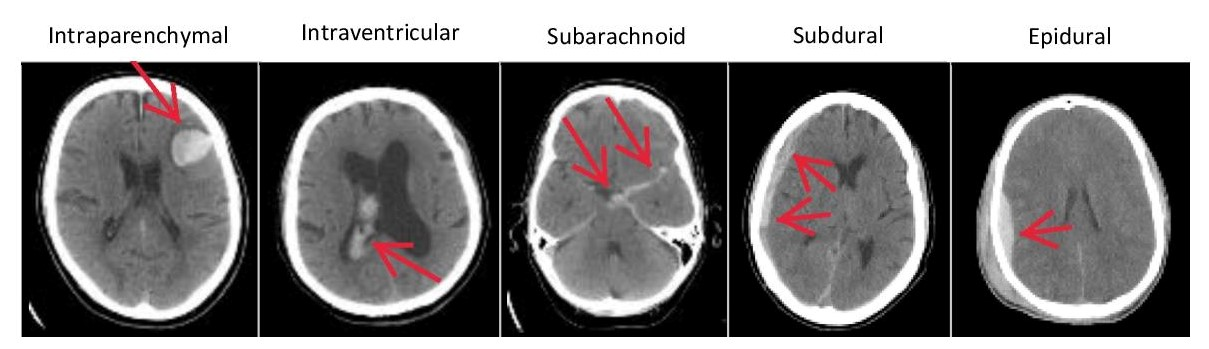
\includegraphics[width=14cm]{assets/images/subtypes}
\par\end{centering}
\caption{Five intracranial hemorrhage subtypes \label{fig:subtypes}}
\end{figure}

The symptoms of the patient and the severity of the bleeding is dependant largely on the subtype. Intraparenchymal hemorrhage is bleeding inside the brain tissue itself, classically centered in the basal ganglia \cite{imagingICH}. It mostly affects patients in the age category from sixty to seventy years. Intraventricular hemorrhage occurs, when the bleeding extends into the ventricles. They are quite uncommon, but can have significantly high mortality rate \cite{neuroimagingInTraumaticImageing}. The third subtype is subarachnoid hemorrhage, which affects the region between the arachnoid and the pia mater. Bleeding in the tissue surrounding the brain is reffered to as extra-axial. Examples of such bleedings are the subdural and epidural subtypes.

\section{Diagnostics}
The current standardized method for diagnosis of intracranial hemorrhage is non-contrast head computer tomography (CT) scanning \cite{imagingICH}. The interpretations of the CT scans are provided by radiologists, however in emergency situations, where quick evaluation is needed, scans are often reviewed by less experienced junior radiologists or attending physicians. A few studies have shown that this can lead to potential misinterpretations, resulting in false diagnosis and even negative consequences on patient's medical condition.  \cite{residentEval, overnightCTinterpret}. In their study, Strub et al. \cite{overnightCTinterpret} concentrated on detecting the rate and cause of errors in interpreting CT scans made by radiology residents, while on call during night shifts. As a result, they stated that misinterpretations of intracranial hemorrhage in head CT scans occur most frquently with subdural and subarachnoid hemorrhage subtypes, in 39\% and 33\% respectively. Overall, out of 22 590 patients' examinations overnight, 1037 discrepancies ensued, 147 of which were cases of intracranial hemorrhage.

Therefore, the motivation of this work is to propose and implement an algorithm, which could potentionally work as an aid-tool to intracranial hemorrhage detection and subtype classification. With such system, the whole process of interpreting CT scans could become more accurate and less faulty.

% Deep learning
\clearpage\null

\chapter{Deep learning}
In this chapter we are going to introduce deep learning, methods of which are going to be implemented in our solution. We will introduce general principles and take a closer look on artificial neural networks, with main focus on convolutional neural networks. Lastly, the topic of interpretability and explainability of neural networks is discussed, with an emphasis on Layer-wise Relevance Propagation.

Deep learning is a form of machine learning, which is a significant part of the scientific field known as artificial intelligence. Over the past decade, a remarkable progress has been made in application of machine learning systems in numerous fields of science as well as in everyday life \cite{longsurvey2018}. They are used in natural language processing, detection of objects in images or speech recognition. These systems thrive mainly because of growing amounts of available data and empowerment of fast GPU computing, both of which is important for their proper training. The usage of machine learning in medicine benefits primarily from ascending volume of digitalized patient data. In 2017 in the United States alone, 150 exabytes of medical data was generated and this number increases annually by approximately 47\% \cite{stanford2017}. With that said, deep learning systems are able to move from theory to practice and assist physicians in hospitals and health centers. According to Stanford Medicine Health Trends Report of 2020 \cite{stanford2020} up to June 2019, the U.S. Food and Drug Administration had approved a total of 46 machine learning algorithms for medical purposes. As machine learning and its applications is still being explored, we can expect this number to further increase rapidly.

Deep learning enables computational models, which are composed of several processing layers, to learn representations of data, which contain multiple  underlying levels of abstraction \cite{greekDeepLearning}. It allows computers to learn from experience and comprehend the world more like a human - as a hierarchy, where complicated concepts are composed of more simple ones. \cite{deeplearningbook} The conventional machine learning approach required a human expert to do a hand-crafted engineering to extract features from data prior to feeding it to a machine, which required much more time and resources. The key advantage of deep learning is that the features are learned by the machine automatically, thanks to a data-driven approach throughout the learning process \cite{deeplearningHealthcare}. 



\section{Deep learning categorization}
We distinguish several primary forms of machine learning, which can be applied to deep learning as well. The main two, which we will discuss in our work, are supervised and unsupervised learning.  \cite{lecundeeplearning} These two forms differ mainly in whether labeled data, corresponding to the input data, is available for the training process. There is a form of learning known as semi-supervised, which we will, however, not further discuss.

\subsection{Supervised learning}
Supervised learning  is the most frequently used form of machine learning \cite{lecundeeplearning}. As it's name suggests, systems which fall under this category are trained under a certain form of supervision, which is present to guide the learning process. During training, a function is computed after each prediction, which measures the error rate of the model. According to the computed value, the internal parameters of the machine are adjusted in order to minimise the error rate in future predictions. These adjustable parameters are the model's most important component. A procedure which empowers nearly all deep learning models' error rate computation and ensures the parameter adjustment is called Stochastic gradient descent. We will discuss this procedure in more detail later in this chapter. Classification and regression are the two main tasks, which supervised learning attempts to solve \cite{kim2019deep}. Our solution will work with labeled data, thus it falls under the category of supervised learning.

\subsection{Unsupervised learning} The technique used by unsupervised learning algorithms is to learn important features contained in the training data without any supervision, as the name implies \cite{deeplearningbook}. Unsupervised learning model attempts to automatically discover the underlying information by extracting and analyzing useful features. This type of learning does not require the training data to be labeled with the correct answer. In this matter embodies it's biggest advantage - withdrawal from the need of labeled data, which would require manual intervention and is not always easy to obtain. Although there is no distinct line between supervised and unsupervised concepts, we can say that the most widely used unsupervised learning algorithms are clustering, principal components analysis, anomaly detection or generative adversarial networks \cite{deeplearningbook, kim2019deep}.

\section{Artificial neural networks}
This section is primarily dedicated to deep neural networks, which are the core of our solution. However, in order to gain better perspective, we will first introduce some conceptual and historical context of artificial neural networks in general.\\
Proposed in the 1940s, artificial neural network (ANN) is a computational model, which is a part of the broad artificial intelligence field. The word "neural" refers to the fact, that it was initially inspired by the way human brain functions. There are approximately $10^{11}$ neurons inside a human brain \cite{navrat2007umela}. Neuron is an elementary cell of the neural system, in which biochemical processes ensure the possibility of processing and sending neural signals. These signals are often referred to as activations. Neurons are interconnected by special joints called synopses, which enables them to communicate \cite{navrat2007umela}. Throughout the whole life, the importance and strength of synopses between neurons change, impacted by human's experience and learning. Artificial neural networks simulate the structure, as well as the behaviour of neurons. If we were to apply the biological terms to an ANN, synopses would be called weights
\subsection*{Perceptron} 
Perceptron is the earliest model of a neural network, composed of a single neuron. The output \textit{o} of the perceptron is defined by the following formula:
\begin{equation}
    o = f(net) = f(\bar w \cdot \bar x) = f (\sum_{j=1}^{n+1} w_jx_j)
\end{equation}
where $f$ is the activation function, $\bar w$ is the weights vector, $\bar x$ is a vector of the input signals. This perceptron calculates with having $n+1$ inputs \cite{navrat2007umela}. The abilities of a single perceptron are quite constrained. It only manages to classify input data into two separate classes. With that said, perceptron provides a solution only to linearly separable problems \cite{navrat2007umela}.
\subsection*{Feedforward neural networks}
Most real-world problems do not have linear character and can not be tackled with the simple perceptron model. A solution to this problem was introduced in 1980s when feedforward neural networks with the backpropagation algorithm were proposed \cite{navrat2007umela}. Multiple neurons (perceptrons) arranged in layers is what constructs a feedforward neural network. In this type of network, the information is passed only in the forward direction and the connections between neurons form a directed acyclic graph. In other words, each neuron from layer \textit{l} sends signals to each neuron in layer \textit{l+1}. The very first (leftmost) layer in a network is called input layer and the last (rightmost) is called output layer. In between, one middle layer, often also called "hidden" layer, is situated. 
\begin{figure}[!ht]
\centering
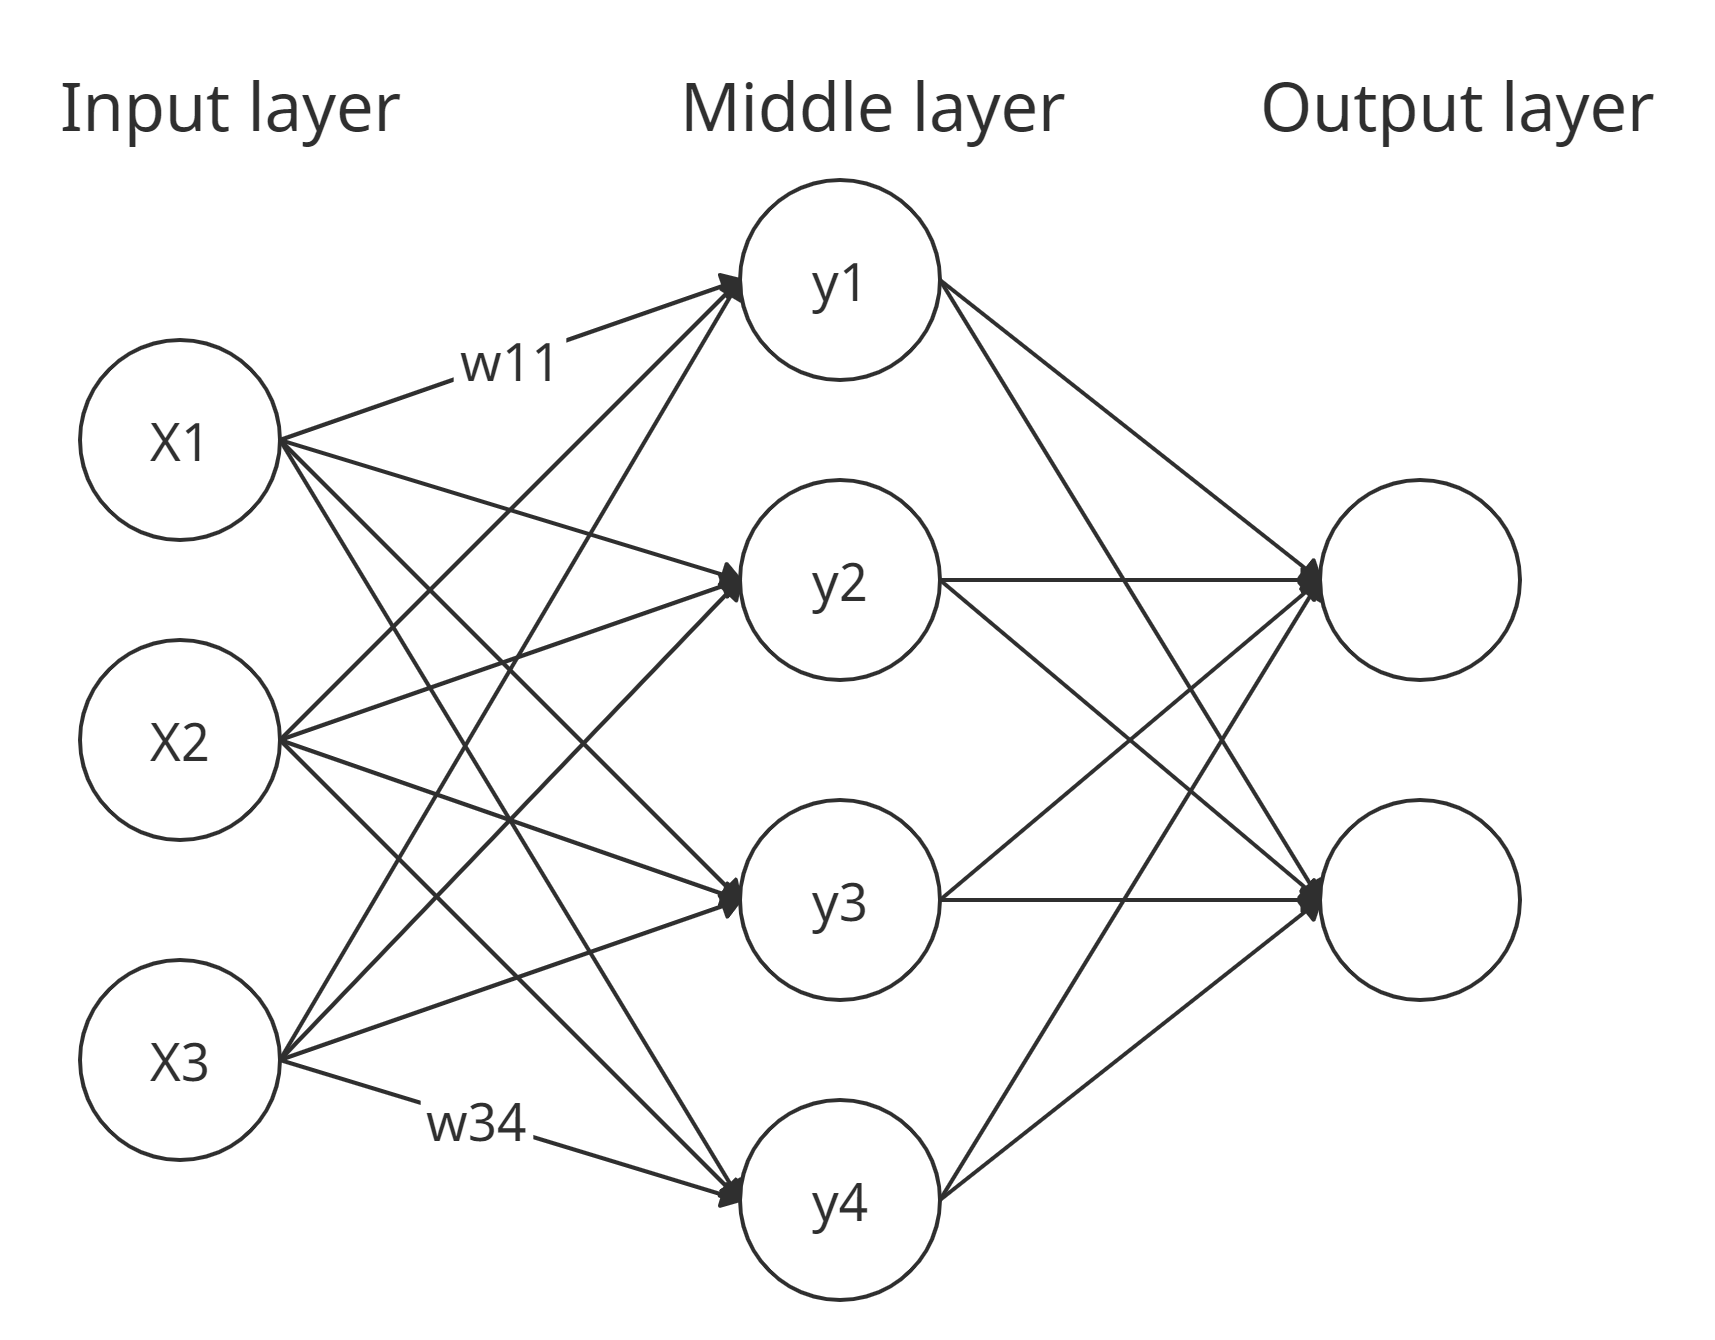
\includegraphics[width=7cm]{assets/images/FFN}
\caption{Architecture of a feedforward neural network
\label{fig:FFN}}
\end{figure}
\\At each layer a calculation is performed, which involves computing a weighted sum of the neuron's input values, followed by a functional operation. Performing this operation equals to applying a nonlinear activation function to the previously computed weighted sum \cite{tutorialIEEE}. The following formula is used at each layer:
\begin{equation}
    y_{j}=f\left({\sum \limits _{i=1}^{n} w_{ij} \times x_{i} + b}\right)
\end{equation}
where $y_j$ is the input value for j-th neuron in corresponding - in this case the middle - layer, $w$ are the weights, $x$ is the value of a neuron from previous layer, $b$ is the bias term and $f$ is the activation function, same as with perceptron mentioned earlier \cite{tutorialIEEE}. The main purpose of bias is to assign each neuron in a network a constant, which would be adjustable by training. The variable $n$ refers to the number of neurons in the previous (input) layer.
\subsection{Deep neural networks}
In the neural networks domain, deep neural networks (DNN) introduce the use of deep learning in a neural network model. This type of neural network differs from the one introduced in previous section in having more than one hidden layer. 
\begin{figure}[!ht]
\centering
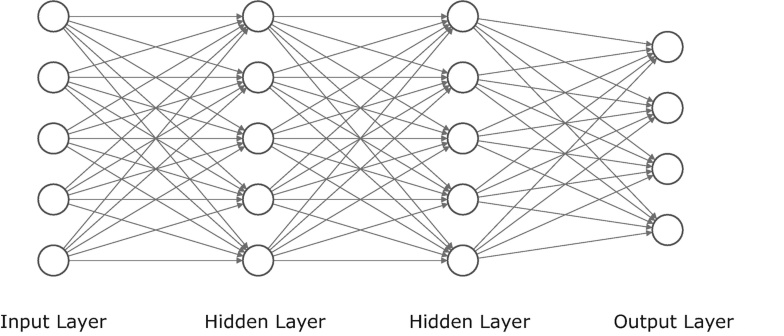
\includegraphics[width=12cm]{assets/images/DNN1}
\caption[Architecture of a deep neural network with two hidden layers]{Architecture of a deep neural network with two hidden layers \footfullcite{chapterBookDL}
\label{fig:DNN}}
\end{figure}

\subsubsection{Activation functions}
For deep neural networks to learn to solve real problem, it is important to introduce nonlinearity into the computational process during training \cite{tutorialIEEE}. This requirement is fulfilled by activation function. There are three historically most frequently used activation functions, each of which is advantageous for a different task.
\begin{figure}[!ht]
\centering
\begin{tikzpicture}
\begin{axis}[
    axis lines=middle,
    xmax=6,
    xmin=-6,
    ymin=-5,
    ymax=5.05,
    xlabel={$x$},
    ylabel={$y$},
    legend pos=north west]
\addplot [domain=-5.5:5.5, samples=100, thick, orange] {max(0, x)};
\addplot [domain=-9.5:9.5, samples=100,
          thick, teal] {1/(1+exp(-x)};
\addplot [domain=-9.5:9.5, samples=100,
     thick, purple] {(exp(x) - exp(-x))/(exp(x) + exp(-x))};
\legend{ReLU, sigmoid, tanh}
\end{axis}
\end{tikzpicture}
\caption{Activation functions graph
\label{fig:activationFunctions}}
\end{figure}
\subsubsection*{Rectified linear function}
Rectified linear or ReLU is the activation function of choice in modern neural networks \cite{tutorialIEEE}. It is defined as:
\begin{equation}
     f(x) = max\{0, x\}
\end{equation}
where we can see, that this function outputs zero if $x\leq0$, otherwise the output is $x$ \cite{deeplearningbook}. However, the fact that it automatically maps all negative values to zero results in decreasing the ability of the DNN to learn properly. Due to this issue, several variations of ReLU were proposed, such as leaky ReLU or parametric ReLU \cite{tutorialIEEE}.

\subsubsection*{Sigmoid function}
The sigmoid function takes an input $x$ and suppresses it to a value from range $[0,1]$, as can be seen in its notation:
\begin{equation}
    f(x) = \sigma(x)=\frac{1}{1+e^{-x}}
\end{equation}
Taking into account its output range, sigmoid is especially beneficial to models, which predict a probability.

\subsubsection*{Hyperbolic tangent function}
The hyperbolic tangent function is similar to sigmoid, however its ouput range is wider. 
\begin{equation}
    f(x) = \tanh(x)=\frac{e^x-e^{-x}}{e^x+e^{-x}}
\end{equation}
This function maps the input $x$ into a value from range $[-1,1]$.
\subsubsection{Backpropagation algorithm}
An optimization technique is what powers the deep learning process. When training a network, we want to minimize average loss, which is the difference between desired output and the current output of the network. It is highly dependable on the weights' adjustment. Updating the weights is executed by computing the gradient descent, through the process of backpropagation \cite{tutorialIEEE}.

\subsubsection*{Stochastic gradient descent}
Stochastic gradient descent is probably the most popular algorithm used for optimization. It is based on the simpler Gradient descent algorithm, which uses the computation of the first derivative to find a global minimum of a function \cite{deeplearningbook}. Let $w_ij^t$ be a weight value at a specific time point, $L$ is the loss and $\alpha$ the current learning rate, we can then compute the update value of the weight as follows:
\begin{equation}
w_{ij}^{t+1} = w_{ij}^{t} - \alpha \frac {\partial L}{\partial w_{ij}}   
\end{equation}
Computing the derivative gives the answer to the question of how the model should adjust its parameters in order to improve its predictions. The word "stochastic" refers to the fact, that instead of all data samples, for each iteration only a few samples are randomly selected for the computation.



\subsection{Convolutional neural networks}
Convolutional neural network (CNN) is a special kind of feedforward neural network, where the convolution operation is used instead of classical matrix multiplication \cite{deeplearningbook}. It was introduced as a method of efficiently handling grid-like data such as images and videos, as it is able to successfully capture the spatial and contextual dependencies within these kinds of 
multi-dimensional data. CNNs have been initially inspired by the functioning of primary visual cortex, located in the bottom back area of the brain \cite{deeplearningbook}.
\subsubsection{Layer architecture}
Convolutional neural network comprises three main different kinds of layers, each of which performs a different role: convolutional layer, pooling layer and fully connected layer.
\begin{figure}[!ht]
\centering
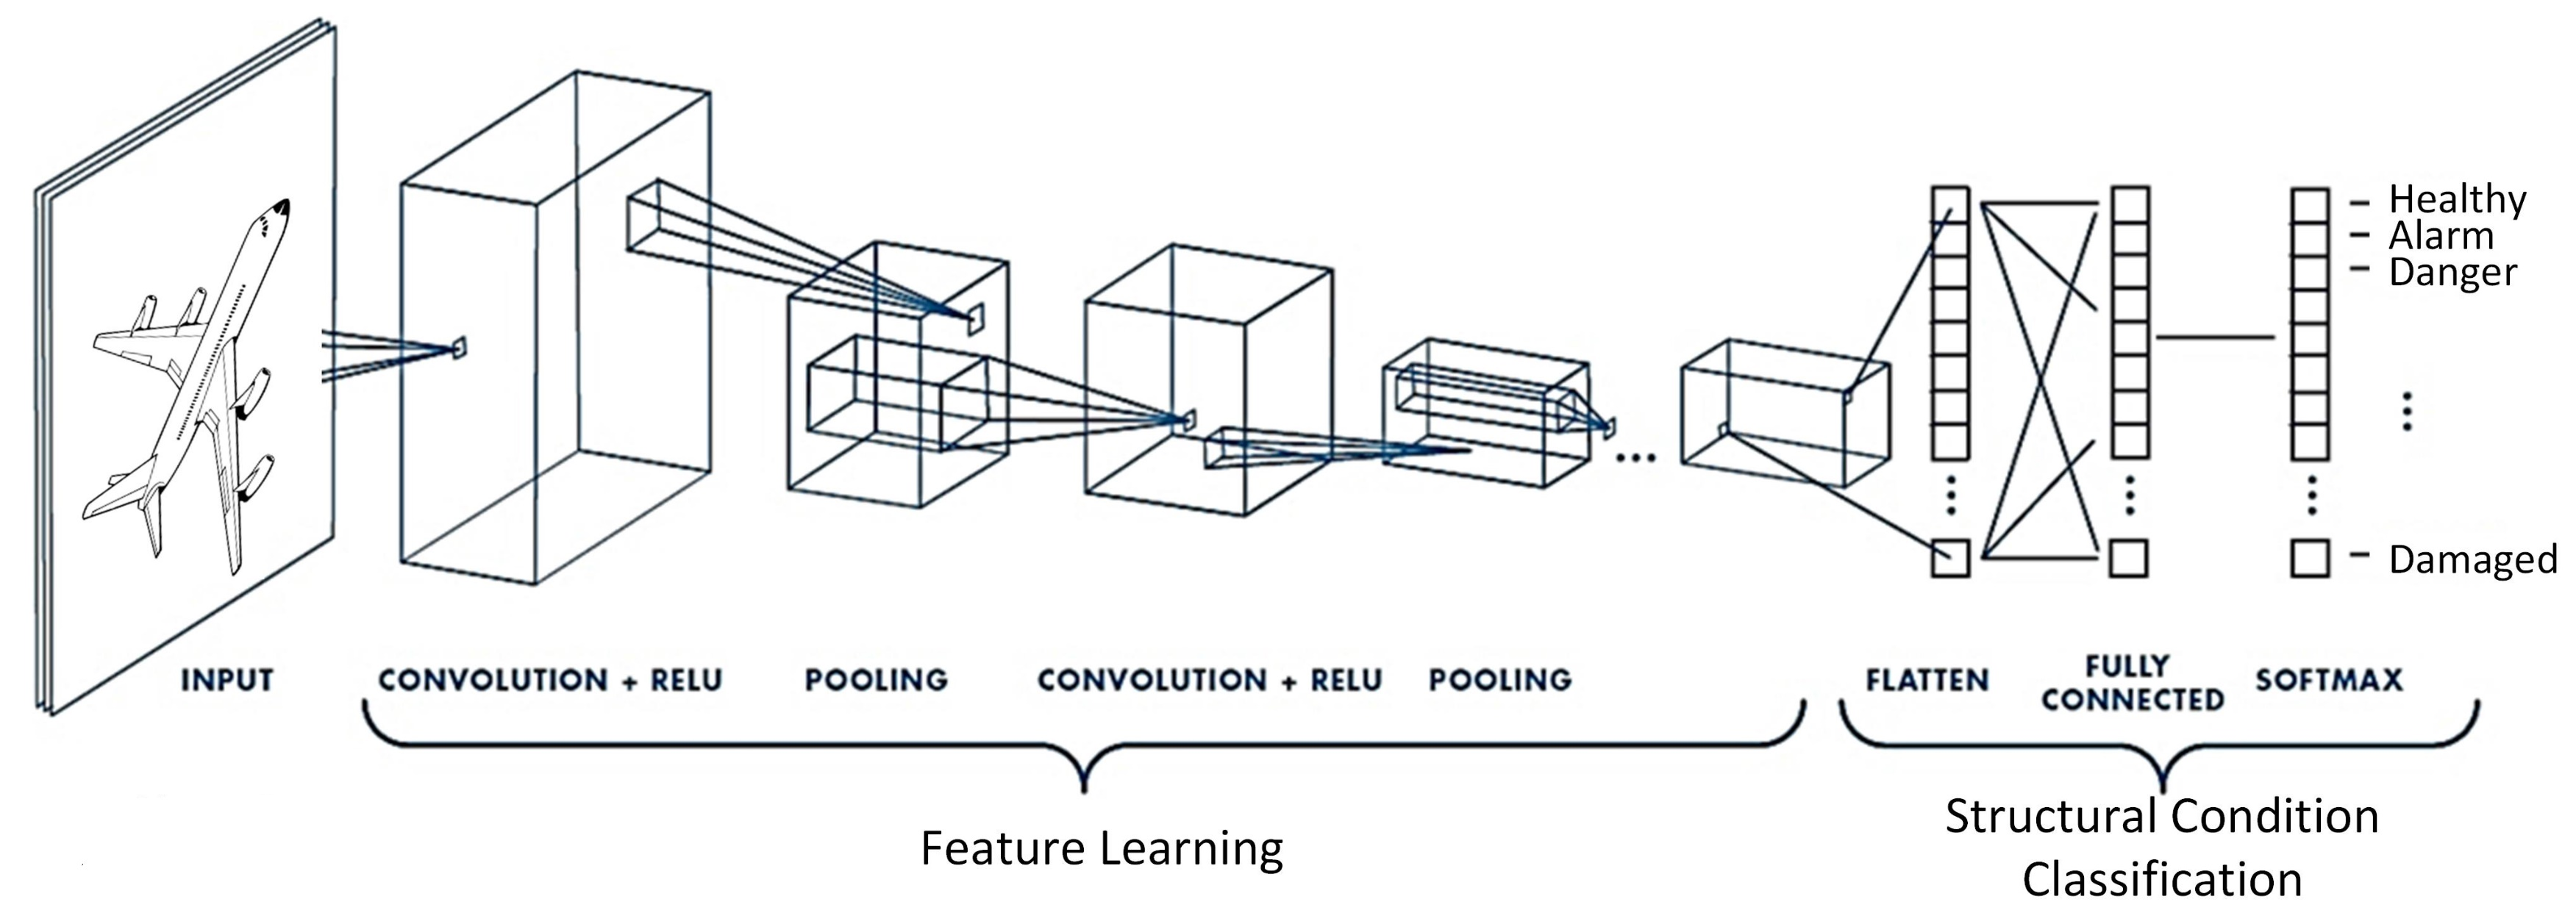
\includegraphics[width=15cm]{assets/images/CNN}
\caption[Example of a convolutional neural network architecture]{Example of a convolutional neural network architecture \footfullcite{CNNpicture}
\label{fig:CNN}}
\end{figure}

\subsubsection*{Convolutional layer}
Convolutional layers are the most important building blocks of a CNN, since they perform the convolution operation, as their name implies. The element accountable for the convolution operation is called a kernel or filter, gradually which slides over the input image. To carry out a convolution basically means to compute matrix multiplication between kernel and the part of the input image, which is currently overlapped by the kernel. As a result of this operation, an output feature map is generated \cite{greekDeepLearning}. The objective of this layer is to detect associations between features passed from the previous layer \cite{lecundeeplearning}. After each convolution layer an activation function, such as ReLU, is applied to introduce nonlinearity.

\subsubsection*{Pooling layer}
A convolutional layer is typically followed by pooling layer. We use pooling to reduce the spatial dimensions through down-sampling of the feature maps. It also enables the network to be invariant to small translations \cite{deeplearningbook}. Different strategies of pooling can be used, namely max pooling or average pooling, returning either the maximum value or the average value from the part of the feature map covered by the kernel respectively \cite{lecundeeplearning}.
\subsubsection*{Fully connected layer}
After several stagies of convolutional a pooling layers, fully connected layer is the one which performs the high-level feature reasoning. In other words, this layer combines features detected in previous layers and thus learns the nonlinear representations in data \cite{greekDeepLearning}. In order to present a 1D vector as the final output, the 2D feature maps are flattened. This flattened vector is then either classified using the softmax classification technique or used for further processing.
\subsubsection{Main concepts}
CNNs greatly benefit from three main concepts: sparse connectivity, equivariant representations and shared parameters. We will discuss each of these separately.
\subsubsection*{Sparse connectivity}
The main motive of sparse connectivity (also sometimes referred to as sparse weights) is the absence of the traditional scheme of connecting each neuron from one layer to each neuron in the previous layer, as it was introduced in traditional feedforward networks \cite{chapterBookDL}. A neuron in convolutional network only interacts with a few other neurons, which can significantly reduce memory requirements as well as improve computational efficiency \cite{deeplearningbook}. In CNN this concept is secured by using a kernel (filter) of a smaller size compared to the size of the input data. Even though the connections in CNN are sparse, neurons in deeper layers are able to interact with input values indirectly. Moreover, deeper situated neurons have larger receptive field compared to neurons in shallow layers, which empowers the network to "efficiently describe complicated interactions between many variables by constructing such interactions from simple building blocks that each describe only sparse interactions" \cite{deeplearningbook}.
\subsubsection*{Shared parameters}
Sparse connectivity closely relates with another concept called shared parameters. It refers to reusing the same set of weight values when calculating the output for a set of neurons \cite{greekDeepLearning}. From the learning point of view, using shared parameters equals to learning only one set of parameters, instead of a separate one for every location of the input \cite{deeplearningbook}. The neurons in a layer that share the same set of weights form a plane. Each plane is then responsible for learning a specific feature \cite{greekDeepLearning}. This concept can reduce memory consumption as well.
\subsubsection*{Equivariant representations}
The last concept, which we will introduce, is equivariant representations, or equivariance in translation. It ensures, that if an input image is changed by any action, the output, generated by convolution operation, changes equivalently to the distortion \cite{deeplearningbook}. This is caused by previously mentioned concept of parameter sharing. Common mathematical definition for equivariance to translation is $f(g(I)) = g(f(I))$, where $I$ represents the input image, $g$ stands for the function executing a distortion and $f$ is the convolution operation.

\section{Interpretability and explainability of neural networks}
As machine learning models constantly work forward and excel in many tasks, a question regarding their trust and transparency arose. They are commonly being addressed as "black boxes", due to the fact, that their arrival at predictions is highly non-transparent \cite{explainDLbook}. In some areas of AI applications, namely those which are part of basic everyday life, such as entertainment or e-commerce, the potential failure of these ML models is rather insignificant, without any serious consequences. However, this can not be applied to domains such as medicine and healthcare, where the life of patients' is at stake. The field of explainable artificial intelligence is dedicated to addressing this challenge \cite{explainDLbook}. For implementing AI models into clinical routine, where they usually maintain a supportive role in the diagnostics process, it is crucial to provide physicians explanation of the model's prediction, to gain more trust and reliability. We will now take a closer look on one of the methods recently explored in explainability of deep learning models.
\subsection{Layer-Wise Relevance Propagation}
Layer-wise Relevance Propagation (LRP) is an algorithm, used in general neural network structures to introduce explainability. In \cite{explainDLbook} it is stated, that "LRP explains individual decisions of a model by propagating the prediction from the output to the input using local redistribution rules". It simply means, that after the neural network makes a prediction, a backward pass through its neurons is conducted, and neurons, which contributed the most to the prediction, are identified \cite{explainDLbook}. As a result a heatmap with most important pixels highlighted is generated.
If $j$ and $k$ are neurons at two neighbouring layers of a neural network, $z_jk$ poses the extent to which neuron j has contributed to make neuron k relevant, then $(R_k)_k$, which is the relevance score at a given layer propagated onto neurons from the lower layer, can be achieved by applying following formula \cite{explainDLbook}:
\begin{equation}
 R_j = \sum _k \frac{z_{jk}}{\sum _{j} z_{jk}} R_k   
\end{equation}

\begin{figure}[!ht]
\centering
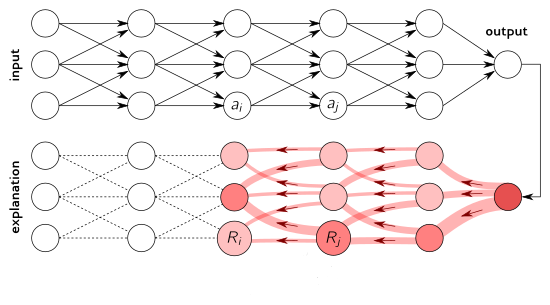
\includegraphics[width=10cm]{assets/images/LRP}
\caption[The LRP procedure]{The LRP procedure \protect\footnotemark}
\end{figure}
\footnotetext{www.heatmapping.org}





% Medical imaging
\clearpage\null
\chapter{Overview of medical imaging}
In this chapter we are going to present a brief overview of medical imaging. First we explore the history of this field, from the 1960s to the current state. Since the aim of this work is detection and classification, we provide a review of approaches to classification task. Lastly, for better understanding of our work and the data we are working with, brief survey of computed tomography is introduced.

Medical imaging, also referred to as radiology, is the medical field which includes the production, as well as analysis and processing of medical image data \cite{diagnostic50years}. Medical professionals use methods of medical imaging, such as computed tomography (CT), magnetic resonance (MRI) or ultrasound, to depict various body parts for diagnostic purposes. With the arrival of digital era it became possible to scan and store significant amounts of medical images digitally. Over the last few decades, researchers have implemented systems to automate the analysis of medical images and it has become one of the main research subjects in the medical imaging field. 

\section{Computer-aided diagnosis}
Initially used approaches in the 1960s resided in construction of rule-based systems, which were able to solve only specific tasks \cite{surveyOnImageing}. These automated computer diagnosis systems brought the very concept of automated diagnostics. It was assumed, that they could potentially completely replace radiologists, believing that computers can achieve better performance at specific tasks, lacking the human-like disposition to making errors. However, with this goal, meeting the expectations on specificity and sensitivity of the systems was simply unattainable, since it required huge amounts of computational power, which was hard to ensure at that time. Thus, in the 1980s the direction of the medical imaging evolution was changed and another approach was presented - computer aided diagnosis (CAD) \cite{diagnostic50years}. The essence of CAD is to improve diagnostic accuracy by assisting radiologists and act as a "second opinion" \cite{surveyOnImageing, CADinmedicalImaging} to their own medical opinion. 
The progress of technology and easier access to high-performance hardware components such as central processing units (CPU) and graphics processing units (GPU) at the end of 1990s resulted in supervised machine learning systems becoming very popular in CAD \cite{surveyOnImageing}. This was viable also due to increasing amount of available medical data (big data), making it possible to train such systems. It was a big step, shifting from completely human designed systems, to ones based on manual feature extraction and then trained automatically by computers. Feature extraction lies at the heart of a successful medical image analysis, therefore the next course of action was to apply machine learning in a self-taught manner for this task as well. We provide more detailed review on deep learning in chapter 4.

% https://ieeexplore.ieee.org/abstract/document/7404017
% http://www.bioscience.org/2019/v24/af/4725/fulltext.php?bframe=2.htm
% https://link.springer.com/article/10.1007%2Fs12194-017-0406-5
% https://www.researchgate.net/profile/Niall_O_Mahony/publication/331586553_Deep_Learning_vs_Traditional_Computer_Vision/links/5cc8bfac4585156cd7bdb5ac/Deep-Learning-vs-Traditional-Computer-Vision.pdf
% https://www.sciencedirect.com/science/article/pii/S093938891830120X
% https://europepmc.org/article/med/28301734#R1
% https://ieeexplore.ieee.org/abstract/document/8241753
% https://www.ncbi.nlm.nih.gov/pmc/articles/PMC1955762/
% https://iopscience.iop.org/article/10.1088/0031-9155/51/13/R02/meta


\section{Computed tomography}
Neuroimaging is crucial when aiming for an exact diagnosis of intracranial hemorrhage.  Taking into account its wide availability and non-invasive technique, computed tomography (CT) is most commonly used in detection of intracranial hemorrhage these days \cite{imagingICH}. Even though magnetic resonance imaging (MRI) has been proven to be more sensitive, CT is able to provide much faster results, which is critical when it comes to obtaining early assessment of the presence and extent of the bleeding \cite{imagingAfterBrainInjury}. The main principle of non-contrast computed tomography imaging resides in the fact, that different tissues of the human body can absorb different amounts of X-ray beams, which is referred to as tissue density \cite{principlesOfCT}. The absorbed X-ray is being mapped into Hounsfield Units (HU). Resulting scans are formed from units of space within the patient's body called voxels. These units contain a three-dimensional (3D) information about the value of tissue density. Resulting 3D scans are studied using a method called windowing, which converts selected range of Hounsfield Units (HU) into values of grayscale (range between 0 and 255).  As a result, a two-dimensional cross sectional "slice" can be extracted from the 3D volume. The selected range is set by two different parameters: window width (WW) and window level (WL). Windowing enables radiologists to study different features and tissues by increasing the contrast, thus bringing forward the tissue of interest \cite{windowClassBiomArt}. The original CT pixel values, which are not in the selected range, are displayed either as black or white, as shown in Figure 3.1 .

\begin{figure}[h]
\begin{centering}
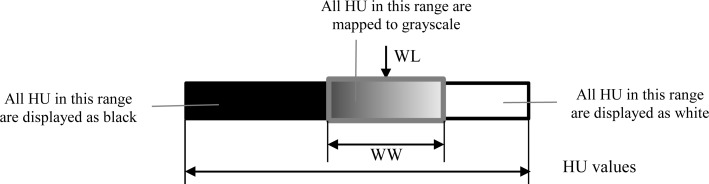
\includegraphics[width=15cm]{assets/images/windowingHU}
\par\end{centering}
\caption{Windowing of CT scans
\label{fig:windowing} \footfullcite{windowClassBiomArt}}
\end{figure}

In detection of intracranial hemorrhage from head CT scans, blood and brain windows are the standard choice. Right after the appearance of hemorrhage, the area of the bleeding shows density values of 60 to 80 Hounsfield units (HU), and as it matures, the value increases up to 100 HU  \cite{principlesOfCT}, which can be visible in the scan slice with a correct setting of window width and window length.

\section{Deep learning in medical imaging}
% https://med.stanford.edu/content/dam/sm/dbds/documents/biostats-workshop/s41591-018-0316-z.pdf
% https://www.ncbi.nlm.nih.gov/pmc/articles/PMC6945006/#b1-ns-1938396-198
\subsection{Detection}
\subsection{Classification}
\subsection{Segmentation}

% Related Work
\clearpage\null
\chapter{Related work}
In this chapter I would like to introduce some related works, in which the authors propose different approaches to the problem of detection and classification of intracranial hemorrhage in non-contrast CT scans.

\section{Identification of intracranial hemorrhage with clinical workflow integration}
 
In their work \cite{relatedWork1} Arbabshirani et al. developed a machine learning algorithm, which automatically analyzed head CT scans, flagging those with the presence of a hemorrhage, and thus prioritized radiology work lists in real time. As a result, the average time, in which a patient received their diagnosis, had been significantly reduced.  

The machine learning algorithm implemented by the authors was a three-dimensional convolutional neural network, which had five convolutional layers and two fully connected layers. The dataset used in development of the solution contained 46 583 non-contrast head CT studies, each having 20 axial two-dimensional slices. Each study had been manually labeled with a binary value, signalizing the presence of a hemorrhage. These labels were later used as ground truths during training period. Prior to the network training, the data had been preprocessed with several techniques, such as standardizing the number of axial slices and resizing each slice, so to achieve a uniform dimensions of 256x256x24, as well as applying windowing, in order to increase the contrast in each of the slices. Thenceforth, the neural network was trained using stochastic gradient descent, until the received loss was near zero. After the training period, the algorithm was tested on previously unseen test data.
Over a three-month period, the trained model had been implemented at a clinic in Pennsylvania, USA to assist with prioritization of radiology work lists. During this implementation phase, 347 head CT studies were processed in real time. For each study, which was fed to the algorithm, a binary output was produced, representing positive or negative presence of ICH. Studies marked as positive were assigned higher priority and moved up the radiology work list. Out of these 94 studies, 60 were determined by a interpreting radiologist as true positive, which gave the model positive predictive value of 64\%. were consequently . With this approach, average diagnostic time was shortened from 8,5 hours to just 19 minutes, which is acceleration of 96\%. The algorithm showed accuracy of 84\% sensitivity of 70\%  and specificity of 87\%. The area under the curve of the model, was established to be 0.846.

\begin{figure}[h]
\begin{centering}
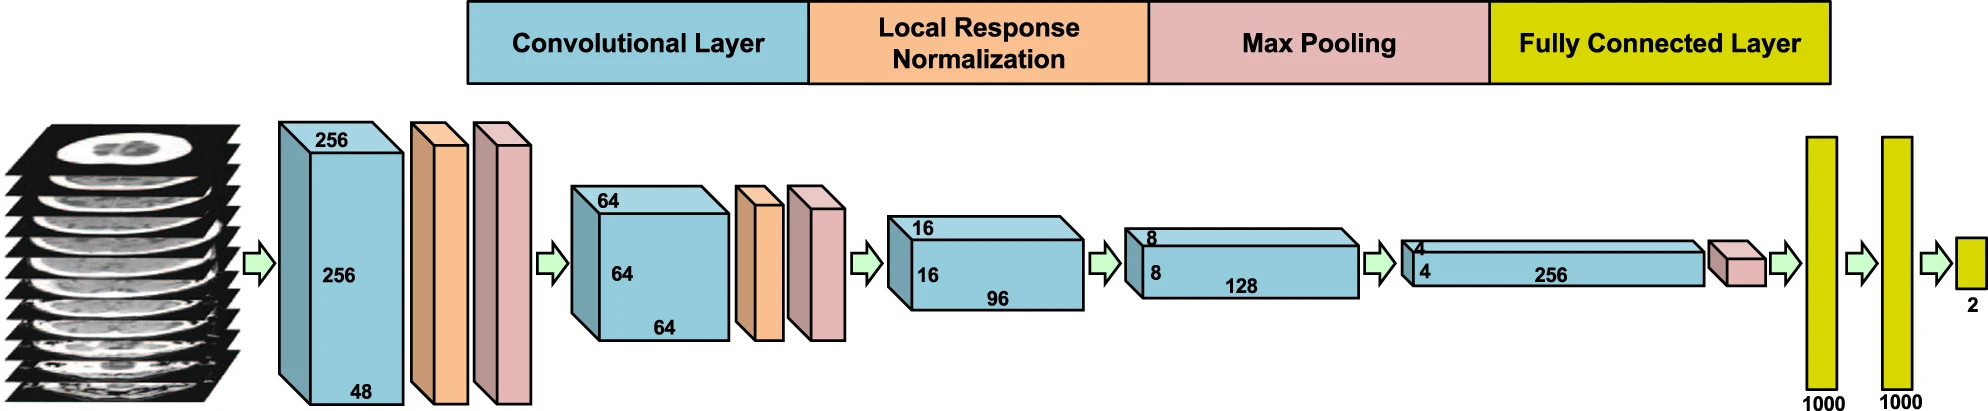
\includegraphics[width=16cm]{assets/images/RW1-net-arch.png}
\par\end{centering}
\caption{Model architecture from \cite{relatedWork1} \label{fig:rw1}}
\end{figure}


\section{Diagnosis of intracranial hemorrhage and subtypes using a three-dimensional joint convolutional and recurrent neural network}

The work of Ye et al. \cite{relatedWork2} resides in combining three-dimensional joint convolutional neural network (CNN) and recurrent neural network (RNN) for the task of detecting intracranial hemorrhage, as well as its five subtypes. The authors conducted a comparison and evaluation of their solution on both slice-level and subject-level (whole 3D CT scan) approaches.

Dataset containing 2836 non-contrast head CT scans was used, with 1836 scans with positive appearance of intracranial hemorrhage. The remaining 1000 scans had been labeled as healthy, without any hemorrhage. All of the scans were labeled on both, slice - and subject - levels. Typically, data preprocessing forewent the training process. This included resampling and downsampling the original dimensions of the scans. Just like in the previously mentioned study \cite{relatedWork1}, different types of windowing were applied on slice-level. Peprocessed data were then used in two stage training. During the first stage, a two-type classification was conducted, which predicted the very presence of a bleeding. With this step, every subject not containing intracranial hemorrhage was filtered out, and only the subjects with bleeding occuring were forwarded to the second stage. In this stage, five-type classification determined the subtype of the hemorrhage present in the scan.

The convolutional neural network was trained to serve as a feature extractor on a slice level. Followed by a reccurent neural network, which was implemented to capture "sequential information of features from consecutive slices, adding inter-slice dependency context to boost classification performance" \cite{relatedWork2}.


% Concept of our solution, preliminary experiments and future work
\clearpage\null
\chapter{Proposed solution} %\label{cha:eva}}




% Resume
\clearpage\null

\chapter*{Plan of the work}
\label{chap:plan}
\addcontentsline{toc}{chapter}{\nameref{chap:plan}}

\section*{Winter semester 2020}

\begin{tabular}{ |c|m{12cm}| } 
 \hline
 Date & Activity \\
 \hline
 \hline
 21.9. - 27.9. & Acquaint with the topic of the work\\ 
 \hline
 28.9. - 4.10. & Challenge and dataset selection \\ 
 \hline
 5.10. - 11.10. & Challenge and dataset selection \\ 
 \hline
 12.10. - 18.10. & Downloading and storage of data, studying literature \\ 
 \hline
 19.10. - 25.10. & Literature research\\ 
 \hline
 26.10. - 1.11. & Studying literature, exploratory data analysis \\ 
 \hline
 2.11. - 8.11. & Studying related work, exploratory data analysis \\
 \hline
 9.11. - 15.11. & The creation of the thesis structure, literature research and study \\ 
 \hline
 16.11. - 22.11. & Writing the analysis (related work), data visualisation \\ 
 \hline
 23.11. 29.11. & Writing the analysis (motivation, medical imaging), studying literature \\ 
 \hline
 30.11. - 6.12. & Writing the analysis (deep learning), deep learning tutorials \\ 
 \hline
 7.12. - 13.12. & Writing the analysis (deep learning), studying deep learning in Python \\ 
 \hline
 14.12. - 20.12. & Writing the analysis (concept), first experiments \\ 
 \hline
 21.12. - 27.12 & Writing the analysis (other parts), first experiments \\ 
 \hline
 28.12. - 3.1.2021 & Finalizing the analysis \\ 
 \hline
\end{tabular}







% Bibliography
\clearpage\null
\printbibliography[heading=references,segment=\therefsegment, resetnumbers=true]

\end{refsegment}

% % Appendix
% \appendix

% \clearpage\null
% \setcounter{figure}{0}
\setcounter{listing}{0}

\chapter{First Appendix \label{cha:chapter1} }

% \begin{refsegment}

% % Appendix
% % \input{appendices/chapter1}

% % Bibliography
% % \printbibliography[heading=referencessec,segment=\therefsegment,resetnumbers=true]

% \end{refsegment}

% \clearpage\null
% \chapter{Contents of Included CD–ROM \label{cha:cdrom} }

CD–ROM included to the thesis contains following files:

\begin{itemize}
\item \texttt{/file1} --- First file
\item \texttt{/file2} --- Second file
\end{itemize}


\end{document}
